\documentclass{article}

\usepackage{fancyhdr}
\usepackage{extramarks}
\usepackage{amsmath}
\usepackage{amsthm}
\usepackage{amsfonts}
\usepackage{tikz}
\usepackage[plain]{algorithm}
\usepackage{algpseudocode}
\usepackage{graphicx}
\usepackage{gensymb}
\usepackage[framed,numbered,autolinebreaks,useliterate]{mcode}
\usepackage{listings}
\usepackage{hyperref}

\graphicspath{{./images/}}

\usetikzlibrary{automata,positioning}

%
% Basic Document Settings
%

\topmargin=-0.45in
\evensidemargin=0in
\oddsidemargin=0in
\textwidth=6.5in
\textheight=9.0in
\headsep=0.25in

\linespread{1.1}

\pagestyle{fancy}
\lhead{\hmwkAuthorName}
\chead{\hmwkClassShort\ \hmwkTitle}
\rhead{\firstxmark}
\lfoot{\lastxmark}
\cfoot{\thepage}

\renewcommand\headrulewidth{0.4pt}
\renewcommand\footrulewidth{0.4pt}

\setlength\parindent{0pt}

%
% Create Problem Sections
%

\newcommand{\enterProblemHeader}[1]{
    \nobreak\extramarks{}{Problem {#1} continued on next page\ldots}\nobreak{}
    \nobreak\extramarks{{#1} (continued)}{{#1} continued on next page\ldots}\nobreak{}
}

\newcommand{\exitProblemHeader}[1]{
    \nobreak\extramarks{{#1} (continued)}{{#1} continued on next page\ldots}\nobreak{}
    % \stepcounter{#1}
    \nobreak\extramarks{{#1}}{}\nobreak{}
}

\setcounter{secnumdepth}{0}
\newcounter{partCounter}

\newcommand{\problemNumber}{0.0}

\newenvironment{homeworkProblem}[1][-1]{
    \renewcommand{\problemNumber}{{#1}}
    \section{\problemNumber}
    \setcounter{partCounter}{1}
    \enterProblemHeader{\problemNumber}
}{
    \exitProblemHeader{\problemNumber}
}

%
% Homework Details
%   - Title
%   - Class
%   - Author
%

\newcommand{\hmwkTitle}{Week\ \#5 Assignment}
\newcommand{\hmwkClassShort}{RBE 595}
\newcommand{\hmwkClass}{RBE 595 --- Reinforcement Learning}
\newcommand{\hmwkAuthorName}{\textbf{Arjan Gupta}}

%
% Title Page
%

\title{
    \vspace{2in}
    \textmd{\textbf{\hmwkClass}}\\
    \textmd{\textbf{\hmwkTitle}}\\
    \vspace{3in}
}

\author{\hmwkAuthorName}
\date{}

\renewcommand{\part}[1]{\textbf{\large Part \Alph{partCounter}}\stepcounter{partCounter}\\}

%
% Various Helper Commands
%

% Useful for algorithms
\newcommand{\alg}[1]{\textsc{\bfseries \footnotesize #1}}

% For derivatives
\newcommand{\deriv}[2]{\frac{\mathrm{d}}{\mathrm{d}#2} \left(#1\right)}

% For compact derivatives
\newcommand{\derivcomp}[2]{\frac{\mathrm{d}#1}{\mathrm{d}#2}}

% For partial derivatives
\newcommand{\pderiv}[2]{\frac{\partial}{\partial #2} \left(#1\right)}

% For compact partial derivatives
\newcommand{\pderivcomp}[2]{\frac{\partial #1}{\partial #2}}

% Integral dx
\newcommand{\dx}{\mathrm{d}x}

% Alias for the Solution section header
\newcommand{\solution}{\textbf{\large Solution}}

% Probability commands: Expectation, Variance, Covariance, Bias
\newcommand{\E}{\mathrm{E}}
\newcommand{\Var}{\mathrm{Var}}
\newcommand{\Cov}{\mathrm{Cov}}
\newcommand{\Bias}{\mathrm{Bias}}

\begin{document}

\maketitle

\nobreak\extramarks{Problem 1}{}\nobreak{}

\pagebreak

\begin{homeworkProblem}[Problem 1]
    When is it suited to apply Monte-Carlo to a problem?

    \subsection{Answer}

    Monte-Carlo methods are best suited to be applied to problems where we do not have a
    model of the environment (i.e., the dynamics of the environment are unknown).
    For example, sometimes it is simply not practical to model
    the complexity of the environment.
    In such cases, the agent must learn about the environment by interacting
    with it and using the obtained rewards to update its policy via the action-value function.\\

\end{homeworkProblem}

\nobreak\extramarks{Problem 2}{}\nobreak{}

\pagebreak

\begin{homeworkProblem}[Problem 2]
    When does the Monte-carlo prediction performs the first update?

    \subsection{Answer}

    The Monte-Carlo prediction performs the first update after an episode terminates. This is because
    the Monte-Carlo method is an episodic method, i.e., it learns from a series of state, action, and reward
    tuples that occur in an episode.\\
\end{homeworkProblem}

\nobreak\extramarks{Problem 2}{}\nobreak{}

\pagebreak

\nobreak\extramarks{Problem 3}{}\nobreak{}

\begin{homeworkProblem}[Problem 3]
    What is off-policy learning and why it is useful?

    \subsection{Answer}

    Off-policy learning is a method of reinforcement learning where the agent learns about the environment
    by observing the behavior of another agent, called the \textit{behavior policy}, which is the policy
    responsible for exploration and interaction. However, the agent
    performs evaluation and optimization using a different policy, called the \textit{target policy}.\\

    Off-policy learning is useful for the following reasons,
    \begin{itemize}
        \item It avoids the unlikely assumption of exploring starts. In some Monte Carlo algorithms, the
        exploratory behavior comes from random starting states, however this is not always possible. Off-policy
        learning allows the agent to learn about the environment without this assumption.
        \item Existing knowledge can be leveraged by learning from the behavior of other agents. The behavior
        policy can be a simple random policy, or it can be a policy that has been learned from past experience.
        \item It avoids the situation where the agent is stuck in a suboptimal policy because it is not 
        exploring enough. This would happen if the agent is using a greedy and deterministic policy to learn about the
        environment.
        \item It avoids unexpected actions that may occur during exploration. 
        Instead, the behavior policy can continuously explore while the target policy learns. This is particularly
        useful in cases where the environment is dangerous or expensive to explore, or if humans are involved.
    \end{itemize}
\end{homeworkProblem}

\pagebreak

\nobreak\extramarks{Problem 4}{}\nobreak{}

\begin{homeworkProblem}[Problem 4]
    \textbf{(Exercise 5.5, page 105)}
    Consider an MDP with a single nonterminal state and a single action
    that transitions back to the nonterminal state with probability $p$ and transitions to the
    terminal state with probability $1-p$. Let the reward be +1 on all transitions, and let
    $\gamma = 1$. Suppose you observe one episode that lasts 10 steps, with a return of 10. What
    are the first-visit and every-visit estimators of the value of the nonterminal state?

    \subsection{Answer}

    Since this problem does not involve a behavior and target policy, we will not use the
    importance sampling ratio. Instead, we can manually calculate the first-visit and every-visit
    estimators of the value of the nonterminal state.\\

    \textbf{Given episode}\\
    
    Let the nonterminal state be $s$ (and let $s_i$ denote the $i^{th}$ time s was visited) 
    and the terminal state be $s'$. Let the action be $a$ (and let $a_i$ denote the $i^{th}$ time s was visited).
    The reward is $r = 1$ for all transitions. Also, $\gamma = 1$.\\

    The given episode is as follows,

    \begin{align*}
        s_0 \xrightarrow{a_1} s_1 \xrightarrow{a_2} s_2 \xrightarrow{a_3} s_3 \xrightarrow{a_4} s_4 \xrightarrow{a_5} s_5 \xrightarrow{a_6} s_6 \xrightarrow{a_7} s_7 \xrightarrow{a_8} s_8 \xrightarrow{a_9} s_9 \xrightarrow{a_{10}} s'
    \end{align*}

    As we can see by the subscript of $a$, there are 10 rewards of $1$ each. Therefore, the total return is $10$.\\

    \textbf{First-Visit Estimator}\\
    The first-visit estimator of the value of the nonterminal state is calculated as follows,

    \begin{align*}
        V(s) &= 1 + 1 + 1 + 1 + 1 + 1 + 1 + 1 + 1 + 1\\
             &= 1(10) = 10
    \end{align*}

    \textbf{Every-Visit Estimator}\\
    The every-visit estimator of the value of the nonterminal state is calculated as follows,

    \begin{align*}
        V(s) &= \frac{1}{10}(1 + 2 + 3 + 4 + 5 + 6 + 7 + 8 + 9 + 10)\\
             &= \frac{1}{10}(55) = 5.5
    \end{align*}

\end{homeworkProblem}

\pagebreak

\nobreak\extramarks{Problem 5}{}\nobreak{}

\begin{homeworkProblem}[Problem 5]
    \textbf{(Exercise 5.7, page 108)}
    In learning curves such as those shown in Figure 5.3 error generally decreases
    with training, as indeed happened for the ordinary importance-sampling method. But for
    the weighted importance-sampling method error first increased and then decreased. Why
    do you think this happened?

    \subsection{Answer}

    As shown in the lectures by Dr. Navid Dadkhah Tehrani, here is a table showing the bias
    and variance comparison between the ordinary importance-sampling method and the weighted
    importance-sampling method.\\

    \begin{center}
        \begin{tabular}{ |c|c|c| } 
            \hline
            & \textbf{Ordinary Importance-Sampling} & \textbf{Weighted Importance-Sampling}\\
            \hline
            Bias & Un-biased & Biased (eventually unbiased)\\
            \hline
            Variance & Large & Low\\
            \hline
        \end{tabular}
    \end{center}

    For weighted importance-sampling, the bias is initially high, but it eventually becomes
    unbiased. That initial bias is what causes the error to increase initially. However, after
    a large number of episodes, the bias decreases and the error decreases as well.\\

    
\end{homeworkProblem}

\pagebreak

\nobreak\extramarks{Problem 6}{}\nobreak{}

\begin{homeworkProblem}[Problem 6]

    \textbf{(Exercise 5.8, page 108)}
    The results with Example 5.5 and shown in Figure 5.4 used a first-visit MC
    method. Suppose that instead an every-visit MC method was used on the same problem.
    Would the variance of the estimator still be infinite? Why or why not?

    \subsection{Answer}

    No, the variance of the estimator would not be infinite. In fact, after the first episode
    that ends with the left action, the value of the state $V(s)$ would be $1$ and would remain
    so for all subsequent episodes.  


\end{homeworkProblem}

\pagebreak

\nobreak\extramarks{Problem 7}{}\nobreak{}

\begin{homeworkProblem}[Problem 7]

    \textbf{(Exercise 3.17)}
    What is the Bellman equation for action values, that
    is, for $q_{\pi}$? It must give the action value $q_{\pi}(s, a)$ in terms of the action
    values, $q_{\pi}(s', a')$, of possible successors to the state-action pair $(s, a)$.\\
    Hint: the backup diagram below corresponds to this equation.
    Show the sequence of equations analogous to (3.14), but for action
    values.

    % \begin{figure}[h!]
    %     \centering
    %     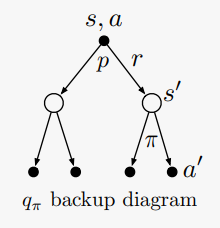
\includegraphics[scale=0.45]{images/suttonbook-qpi-backup-diag.png}
    % \end{figure}

    \subsection{Answer}

    From the textbook, the action-value function for a policy $\pi$ is defined as,

    \begin{align*}
        q_{\pi}(s, a) &\doteq \mathbb{E}_{\pi} \left[ G_t \mid S_t = s, A_t = a \right]\\
                   &= \mathbb{E}_{\pi} \left[ \sum_{k=0}^{\infty} \gamma^k R_{t+k+1} \mid S_t = s, A_t = a \right]\\
                   &= \mathbb{E}_{\pi} \left[ R_{t+1} + \gamma \sum_{k=0}^{\infty} \gamma^k R_{t+k+2} \mid S_t = s, A_t = a \right]\\
                   &= \mathbb{E}_{\pi} \left[ R_{t+1} + \gamma G_{t+1} \mid S_t = s, A_t = a \right]\\
                     &= \mathbb{E}_{\pi} \left[ R_{t+1} \mid S_t = s, A_t = a \right] + \gamma \mathbb{E}_{\pi} \left[ G_{t+1} \mid S_t = s, A_t = a \right]\\
    \end{align*}

    Now, let us consider the first and second terms of the above equation separately.\\

    \textbf{First Term}\\
    \vspace{-0.25cm}
    \begin{align*}
        \mathbb{E}_{\pi} \left[ R_{t+1} \mid S_t = s, A_t = a \right] &= \sum_{r \in \mathcal{R}} r \cdot p(r \mid s, a)
        = \sum_{r \in \mathcal{R}} \sum_{s' \in \mathcal{S}} r \cdot p(s', r \mid s, a)
    \end{align*}

    \textbf{Second Term}\\
    \vspace{-0.25cm}
    \begin{align*}
        \gamma \mathbb{E}_{\pi} \left[ G_{t+1} \mid S_t = s, A_t = a \right] &= \gamma \sum_{g \in \mathcal{G}} g \cdot p(g \mid s, a)\\
        &= \gamma \sum_{g \in \mathcal{G}} \sum_{r \in \mathcal{R}} \sum_{s' \in \mathcal{S}} \sum_{a' \in \mathcal{A}} g \cdot p(g \mid s', a') \cdot p(s', r \mid s, a) \cdot \pi(a' \mid s')\\
    \end{align*}
    Where, $\sum_{g \in \mathcal{G}} g \cdot p(g \mid s', a') = \mathbb{E}_{\pi} \left[ G_{t+1} \mid S_{t+1} = s', A_{t+1} = a' \right] = q_{\pi}(s', a')$\\

    Therefore the second term is,

    \begin{align*}
        \gamma \mathbb{E}_{\pi} \left[ G_{t+1} \mid S_t = s, A_t = a \right] &= \gamma\sum_{r \in \mathcal{R}} \sum_{s' \in \mathcal{S}} \sum_{a' \in \mathcal{A}} q_{\pi}(s', a') \cdot p(s', r \mid s, a) \cdot \pi(a' \mid s')\\
    \end{align*}

    Now, combining the first and second terms, we get,

    \begin{align*}
        q_{\pi}(s, a) &=  \sum_{r \in \mathcal{R}} \sum_{s' \in \mathcal{S}} r \cdot p(s', r \mid s, a) + \gamma\sum_{r \in \mathcal{R}} \sum_{s' \in \mathcal{S}} \sum_{a' \in \mathcal{A}} q_{\pi}(s', a') \cdot p(s', r \mid s, a) \cdot \pi(a' \mid s')\\
        q_{\pi}(s, a) &= \sum_{s',r} p(s', r \mid s, a) \left[ r + \gamma\sum_{a'} \pi(a' \mid s') q_{\pi}(s', a') \right]\\
    \end{align*}

    Which is the Bellman equation for action values, i.e., for $q_{\pi}$.

    \subsubsection{Backup Diagram Confirmation}

    This equation can be verified by looking at the backup diagram given in the prompt. The backup diagram
    shows that we start with the state-action pair $(s, a)$. To get to the next state, we are subjected
    to the environment $p(s', r \mid s, a)$. The reward $r$ is added to the discounted return $G_{t+1}$.
    This brings us to our new state, $s'$. At this point, the equation would look as follows,

    \begin{align*}
        q_{\pi}(s, a) &= \sum_{s',r} p(s', r \mid s, a) \left[ r + \gamma v_{\pi}(s') \right]\\
    \end{align*}

    However we still need to eliminate the $v_{\pi}(s')$ term. To do this, we go through our
    policy, $\pi$, to get the action $a'$ that we would take in the state $s'$. Now the equation
    becomes,

    \begin{align*}
        q_{\pi}(s, a) &= \sum_{s',r} p(s', r \mid s, a) \left[ r + \gamma\sum_{a'} \pi(a'\mid s') q_{\pi}(s', a') \right]\\
    \end{align*}

    So, the Bellman equation for action values, i.e., for $q_{\pi}$, is confirmed by the backup diagram.

\end{homeworkProblem}

\pagebreak

\nobreak\extramarks{Problem 8}{}\nobreak{}

\begin{homeworkProblem}[Problem 8]

    \textbf{(Exercise 3.22)}
    Consider the continuing MDP shown below. The only decision to be made is that in the top state,
    where two actions are available, left and right. The numbers
    show the rewards that are received deterministically after
    each action. There are exactly two deterministic policies,
    $\pi_{\text{left}}$ and $\pi_{\text{right}}$.
    What policy is optimal if $\gamma = 0$? If $\gamma = 0.9$?
    If  $\gamma = 0.5$?

    % \begin{figure}[h!]
    %     \centering
    %     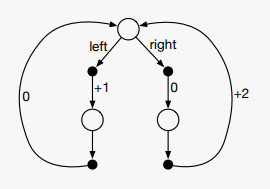
\includegraphics[scale=0.45]{images/suttonbook-ex3.22-fig.png}
    % \end{figure}

    \subsection{Answer}

    The discounted return is defined as,

    \[
    \tag{3.8}
        G_t \doteq R_{t+1} + \gamma R_{t+2} + \gamma^2 R_{t+3} + \cdots = \sum_{k=0}^{\infty} \gamma^k R_{t+k+1}
    \]

    \subsubsection{Case 1: $\gamma = 0$}

    When $\gamma = 0$, the left policy rewards are calculated as follows,

    \begin{align*}
        G_{\text{left}} &= 1 + 0 + 0 + \cdots = 1
    \end{align*}

    Similarly, the right policy rewards are calculated as follows,

    \begin{align*}
        G_{\text{right}} &= 0 + 0 + \cdots = 0
    \end{align*}

    In this case, the \textbf{left} policy is optimal.

    \subsubsection{Case 2: $\gamma = 0.9$}

    When $\gamma = 0.9$, the left policy rewards are calculated as follows,

    \begin{align*}
        G_{\text{left}} &= 1 + 0.9 \cdot 0 + 0.9^2 \cdot 1 + \cdots\\
                        &= 1 + 0.9^2 + 0.9^4 + \cdots\\
                        &= \sum_{k=0}^{\infty} 0.9^{2k}\\
                        &= \sum_{k=0}^{\infty} 0.81^{k}\\
                        &= \frac{1}{1 - 0.81}
                        = \frac{1}{0.19}\\
                        &= 5.263
    \end{align*}

    Similarly, the right policy rewards are calculated as follows,

    \begin{align*}
        G_{\text{right}} &= 0 + 0.9 \cdot 2 + 0 + 0.9^3 \cdot 2 + \cdots \\
                        &= 0.9 \cdot 2 + 0.9^3 \cdot 2 + \cdots\\
                        &= 2 \cdot \sum_{k=0}^{\infty} 0.9^{2k+1}
                        = 2 \cdot \sum_{k=0}^{\infty} (0.9)(0.81)^{k}
                        = 2 \cdot \frac{0.9}{1 - 0.81}\\
                        &= \frac{1.8}{0.19} = 9.474
    \end{align*}

    In this case, the \textbf{right} policy is optimal.

    \subsubsection{Case 3: $\gamma = 0.5$}

    When $\gamma = 0.5$, the left policy rewards are calculated as follows,

    \begin{align*}
        G_{\text{left}} &= 1 + 0.5 \cdot 0 + 0.5^2 \cdot 1 + \cdots\\
                        &= 1 + 0.5^2 + 0.5^4 + \cdots\\
                        &= \sum_{k=0}^{\infty} 0.5^{2k}
                        = \sum_{k=0}^{\infty} 0.25^{k}\\
                        &= \frac{1}{1 - 0.25}
                        = \frac{1}{0.75}\\
                        &= 1.333
    \end{align*}

    Similarly, the right policy rewards are calculated as follows,

    \begin{align*}
        G_{\text{right}} &= 0 + 0.5 \cdot 2 + 0 + 0.5^3 \cdot 2 + \cdots \\
                        &= 0.5 \cdot 2 + 0.5^3 \cdot 2 + \cdots\\
                        &= 2 \cdot \sum_{k=0}^{\infty} 0.5^{2k+1}
                        = 2 \cdot \sum_{k=0}^{\infty} (0.5)(0.25)^{k}
                        = 2 \cdot \frac{0.5}{1 - 0.25}\\
                        &= \frac{1}{0.75} = 1.333
    \end{align*}

    In this case, both the \textbf{left} and \textbf{right} policies are optimal.

\end{homeworkProblem}

\end{document}